\lemma (\textit{О связи частных производных и производных по направлению}) Пусть $G \subset \R^{n}$~---~открытое непустое множество, $f$: $G \mapsto \R$, $x^{0} \in G.$ Тогда верно:
$$\forall i \in \{1, \ldots, n\} \ \exists \dfrac{\partial f}{\partial x_i} (x^0) \Longleftrightarrow \begin{cases}
    \exists \dfrac{\partial f}{\partial l_{i}^{+}} \in \R \\
    \exists \dfrac{\partial f}{\partial l_{i}^{-}} \in \R \\
    \dfrac{\partial f}{\partial l_{i}^{+}} = - \dfrac{\partial f}{\partial l_{i}^{-}}, 
\end{cases}$$ где $l_{i}^{+}$~---~элемент множества $\R^{n},$ у которого $i-$ая компонента равна $1$, то есть\\ $(\underset{1}{0}, \ldots, \underset{i}{1}, \ldots, \underset{n}{0})$, а у $l_{i}^{-}$ -- $(-1).$ Причем  
$$\exists \dfrac{\partial f}{\partial x_i} (x^0) \Longrightarrow \dfrac{\partial f}{\partial x_i} (x^0) = \dfrac{\partial f}{\partial l_{i}^{+}} (x^{0}).$$

\begin{proof}
    Зафиксируем $i \in \{1, \ldots, n\}.$ Рассмотрим функцию $$\varphi(t) := f(x_1^0, \ldots, x_i^0 + t, \ldots, x_n^0).$$ Тогда $$\exists \dfrac{\partial f}{\partial x_i} (x^0) \Longleftrightarrow \exists \frac{d\varphi}{dt}(0) \in \R \Longleftrightarrow \begin{cases}
        \exists \varphi'_{+}(0) \in \R\\
        \exists \varphi'_{-}(0) \in \R \\
        \varphi'_{+}(0) = \varphi'_{-}(0)
    \end{cases}$$
    По определению:
    $$\varphi'_{+}(0) := \lim\limits_{t \to +0} \dfrac{f(x_1^0, \ldots, x_i^0 + t, \ldots x_n^0) - f(x_1^0, \ldots, x_i^0, \ldots x_n^0)}{t} $$
    $$\varphi'_{-}(0) := \lim\limits_{h \to -0} \dfrac{f(x_1^0, \ldots, x_i^0 + h, \ldots x_n^0) - f(x_1^0, \ldots, x_i^0, \ldots x_n^0)}{h} = \ \  \left<h = -t \right> \ \  = $$ $$ = \lim\limits_{t \to +0} \dfrac{f(x_1^0, \ldots, x_i^0 - t, \ldots x_n^0) - f(x_1^0, \ldots, x_i^0, \ldots x_n^0)}{-t}$$
    То есть получим, что:
    $$\varphi'_{+}(0) = \dfrac{\partial f}{\partial l_{i}^{+}}$$
    $$\varphi'_{-}(0) = - \dfrac{\partial f}{\partial l_{i}^{-}}$$
    Объединяя все выше написанное, получаем требуемое.
\end{proof}

%\newpage А зачем..

\begin{theorem}
    Пусть $G \subset \R^{n}$ открытое непустое множество, $f$: $G \mapsto \R$, $x^{0} \in G$ дифференцируема в точке $x^0$. Тогда 
    $$\forall i \in \{1, \ldots, n\} \ \exists \dfrac{\partial f}{\partial x_i} (x^0) = \left( \textup{grad} f(x^0) \right)_i$$
\end{theorem}

\begin{proof}
    На прошлой лекции было доказано:
    $$\exists \dfrac{\partial f}{\partial l} (x^0) = \left( \textup{grad} f(x^0), l\right)$$
    Следовательно:
    $$\forall i \in \{1, \ldots, n\}$$
    $$\exists \dfrac{\partial f}{\partial l_i^{+}} (x^0) = \left( \textup{grad} f(x^0) \right)_i$$
    $$\exists \dfrac{\partial f}{\partial l_i^{-}} (x^0) = -\left( \textup{grad} f(x^0) \right)_i$$
    По только что доказанной лемме, получим требуемое.
\end{proof}

\begin{note}
    Заметим, что мы определяли градиент только для дифференцируемых функций.
\end{note}

\begin{corollary}
    Пусть $G \subset \R$ открытое непустое множество, $f$: $G \mapsto \R^{n}$, $x^{0} \in G$ дифференцируема в точке $x^0.$ Тогда 
    $$d_{x^0}f = \left(\textup{grad}f(x^0), dx \right).$$
\end{corollary}

\begin{theorem}
    (\textit{Достаточные условия дифференцируемости в точке})  Пусть $G \subset \R^{n}$ открытое непустое множество, $f$: $G \mapsto \R$, $x^{0} \in G.$ Пусть $\exists \delta > 0$: $\forall x \in B_{\delta}(x^0) \ \ \forall i \in \{1, \ldots, n\} \ \exists \dfrac{\partial f}{\partial x_i} (x)$, то есть в каждой точке шара существует частная производная и пусть $\dfrac{\partial f}{\partial x_i}$ непрерывна в точке $x^0$ $ \ \forall i \in \{1, \ldots, n\}.$ Тогда $f$ дифференцируема в точке $x^{0}$.
\end{theorem}

\begin{proof}
    Дадим доказательство только в двумерном случае, так как в многомерном доказательстве аналогично.
    
    \sidefig(8.4 cm)(7 cm)
    {
    \begin{flushleft}
    \normalsize Пусть
        $
            \begin{cases}
                x = x^{0} + h_{1}\\
                y = y^{0} + h_{2}
            \end{cases}\hfill\newline
        $
        
        \normalsize Рассмотрим
        $f(x, y) - f(x^0, y^0) = f(x^0 + h_1, y^0 + h_2) - f(x^0, y^0) = \left( f(x^0 + h_1, y^0 + h_2) - f(x^0 + h_1, y^0) \right) + \left( f(x^0 + h_1, y^0) - f(x^0, y^0) \right)\newline$
    \end{flushleft}
    }
    {
    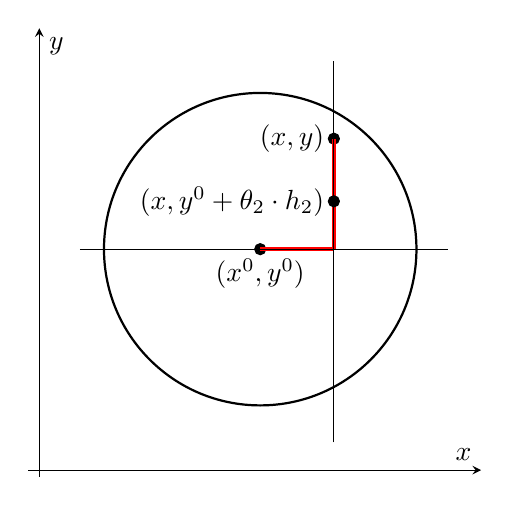
\begin{tikzpicture}[scale=1]
    \begin{axis}[
        axis lines=middle,
        xlabel=$x$, ylabel=$y$,
        xmin=-0.3, xmax=12,
        ymin=-0.175, ymax=12,
        xtick={0},
        ytick={0},
        tick label style={font=\small},
        axis equal image
    ]

    \draw[thick, black](axis cs: 6,6) circle[radius=sqrt(18)];

    \filldraw[black] (axis cs: 6,6) circle (2pt) node[anchor=north]{$(x^{0}, y^{0})$};
    \filldraw[black] (axis cs: 8,9) circle (2pt) node[anchor=east]{$(x, y)$};
    \draw[ultra thick, red] (axis cs: 6,6) -- (axis cs: 8,6);
    \draw[ultra thick, red] (axis cs: 8,6) -- (axis cs: 8,9);
    \draw[thin, black] (axis cs: 8,0.75) -- (axis cs: 8,11.1);
    \draw[thin, black] (axis cs: 1.1,6) -- (axis cs: 11.1,6);
    \filldraw[black] (axis cs: 8,7.3) circle (2pt) node[anchor=east]{$(x, y^{0} + \theta_{2} \cdot h_{2})$};
    
    \end{axis}


\end{tikzpicture}

    }

    Рассмотрим функцию $\phi(t) = f(x^0 + h_1, t),$ она дифференцируема в некотором интервале, который содержит отрезок $[y^0, y^0 + h_2].$ Значит, по теореме Лагранжа
$\exists \psi \in (y^0, y^0 + h): \psi = \theta \cdot h, \  \theta \in (0, 1)$:
    
    $$f(x^0 + h_1, y^0 + h_2) - f(x^0 + h_1, y^0) = \phi'(\psi) \cdot h_2 = \dfrac{\partial f}{\partial y} (x^0 + h_1, y_0 + \theta_2 \cdot h_2) \cdot h_2.$$
    Аналогично, второе слагаемое представим в таком виде. Имеем:
    
    $f(x, y) - f(x^0, y^0) = \dfrac{\partial f}{\partial x} (x^0 + \theta_1 \cdot h_1, y^0) \cdot h_1 + \dfrac{\partial f}{\partial y} (x^0 + h_1, y^0 + \theta_2 \cdot h_2) \cdot h_2 = $
    
    (Мы получили производные в какой-то точке, но мы знаем про точку $(x^0, y^0)$ поэтому добавим и вычтем необходимые слагаемые.)
    
    $ = \left( \dfrac{\partial f}{\partial x} (x^0 + \theta_1 \cdot h_1, y^0) - \dfrac{\partial f}{\partial x} (x^0, y^0) \right) \cdot h_1 + \dfrac{\partial f}{\partial x} (x^0, y^0) \cdot h_1 +  $
    \begin{flushright}
            $+ \left( \dfrac{\partial f}{\partial y} (x^0 + h_1, y^0 + \theta_2 \cdot h_2) - \dfrac{\partial f}{\partial y} (x^0, y^0)\right) \cdot h_2 + \dfrac{\partial f}{\partial y} (x^0, y^0) \cdot h_2$
    \end{flushright}


    В силу непрерывности каждая из скобок является бесконечно малой функцией $(\epsilon_{1, 2}(h_1, h_2) \to 0, (h_1, h_2) \to 0)$. В итоге:
    $$\Delta f = \dfrac{\partial f}{\partial x} (x^0, y^0) \cdot h_1 + \dfrac{\partial f}{\partial y} (x^0, y^0) \cdot h_2 + \left( \epsilon_1(h_1, h_2) \cdot \frac{h_1}{||h||} + \epsilon_2(h_1,h_2) \cdot \frac{h_2}{||h||}\right) \cdot ||h||$$
    Следовательно, по определению дифференцируемости получим требуемое.
    Примечание: вместо $\delta$ шара можно брать куб
\end{proof}

\subsection{Дифференцируемость отображений} 

\begin{definition}
    Пусть $m, n \in \N$, $G \subset \R^{n}$~---~непустое открытое множество, $F$: $G \mapsto \R^{m}.$ Будем говорить, что отображение $F$ дифференцируемо в точке $x^0 \in G,$ если существует линейное отображение $\mathcal{L}$: $\R^n \mapsto \R^m:$
$$F(x) - F(x^{0}) = \mathcal{L}(x-x^0) + \overline{o}(\|x - x^{0}\|)\text{, }x\rightarrow x^{0}.$$ При этом $\mathcal{L}$ будем называть дифференциалом $F$ в точке $x_0$ и обозначать $d_{x^0}F.$ 
\end{definition}

\begin{note}
    Cуществование $\mathcal{L}$ эквивалентно существованию матрицы $A$ размера $m \times n:$
    $$ A = \begin{pmatrix}
  a_{11}& \ldots & a_{1n}\\
  \vdots & \ddots & \vdots \\
  a_{m1}& \ldots & a_{mn}
\end{pmatrix}$$
Задать отображение $F$: $G \mapsto \R^{m} \Longleftrightarrow$ задать $m$ функций, то есть $F = \begin{pmatrix}
    F_{1}\\
    \vdots \\
    F_{m}
\end{pmatrix}$.
\end{note}

\begin{proposition}
    Отображение $F$: $G \mapsto \R^{m}$ дифференцируемо в точке $x^{0} \Longleftrightarrow \forall j \in \{1, \ldots, m\}$ $F_j$ дифференцируема в точке $x^{0}.$ При этом матрица отображения $A$: $A_{ij} = \dfrac{\partial F_i}{\partial x_j} (x^0)$ называют матрицей Якоби отображения (или производной) $F$ в точке $x^{0}$ и обозначают $\D F(x^0)$. 
\end{proposition}

\begin{proof}
    Дифференцируемость отображения $F$ в точке $x^{0}$ по определению равносильна тому, что $\exists \mathcal{L}$: $\R^n \mapsto \R^m$: $F(x) - F(x^{0}) = \mathcal{L}(x - x^{0}) + \overline{o}(\|x - x^{0}\|)$, $x\to x^{0}$. Перепишем в матричном виде 
    $$\begin{pmatrix}
            F_{1} (x) - F_{1} (x^{0})\\
            \vdots\\
            F_{m} (x) - F_{m} (x^{0})
        \end{pmatrix} = 
        \begin{pmatrix}
            a_{11}& \ldots & a_{1n}\\
            \vdots & \ddots & \vdots \\
            a_{m1}& \ldots & a_{mn}
        \end{pmatrix} \cdot \begin{pmatrix}
            x_{1} - x_{1}^{0}\\
            \vdots\\
            x_{n} - x_{n}^{0}
    \end{pmatrix} + \begin{pmatrix}
            o_{1} (\|x - x^{0}\|)\\
            \vdots\\
            o_{m} (\|x - x^{0}\|)
    \end{pmatrix}, \ x\to x^{0} \Longleftrightarrow$$
    $\Longleftrightarrow \forall j \in \{1, \ldots, m\}$ $F_{j}$ дифференцируемо в точке $x^{0}$, при этом $\forall j \in \{1, \ldots, m\}$ строка $(a_{j1}, \ldots, a_{jn}) = \text{grad}F_{j} (x^{0}) = \left(\cfrac{\partial F_{j}}{\partial x_{1}} (x^{0}), \ldots, \cfrac{\partial F_{j}}{\partial x_{n}} (x^{0})\right)$.
\end{proof}

% Крч юзай \D для якобиана, я настроил чтобы красивое было
